\documentclass[12pt]{article}
\usepackage[a4paper]{geometry}
\usepackage[spanish,es-tabla]{babel}
\usepackage[utf8]{inputenc}
\usepackage[T1]{fontenc}
% \usepackage{fontspec}
\usepackage{graphicx}
\usepackage{times}
\usepackage{amsmath}
\usepackage{setspace}
\usepackage{enumitem}
\usepackage{fancyhdr}
\usepackage{lipsum}
\usepackage{parskip}
\usepackage[backend=biber, style=apa]{biblatex}
\addbibresource{references.bib}
\usepackage{caption}
\usepackage{floatrow}
\usepackage{titlesec}
\usepackage{titletoc}
\usepackage{appendix}
\usepackage{tabularray}
\usepackage{tocloft} 
\usepackage{titlesec}
\usepackage{physics}
\usepackage{changepage}
\usepackage[hidelinks]{hyperref} % eliminar rectangulos rojos en los links

\usepackage{titlesec}
\titleformat{\section}
  {\normalfont\fontsize{16}{16}\bfseries}{\thesection .}{0.5ex}{}
\titleformat{\subsection}
  {\normalfont\fontsize{14}{14}\bfseries}{\thesubsection .}{0.5ex}{}
\titleformat{\subsubsection}
  {\normalfont\fontsize{14}{14}\bfseries}{\thesubsubsection.}{0.5ex}{}


%-----------------CONFIGURACION-------------------------------

% Configuracion de la Pagina 
\geometry{
    a4paper,
    total={21cm,29.7cm},
    left=3cm,
    top=2.5cm,
    right=2.5cm,
    bottom=2.5cm }

\setstretch{1.5} %Interlineado a 1.5
\setlength{\parindent}{1cm} %Sangría de cada nuevo párrafo a 1cm

% Configuración del pie de página
\fancyfoot[C]{\rule{\textwidth}{0.4pt}\\ \hspace*{\fill}\fontsize{12pt}{14pt}\selectfont Título de Tesis \hspace*{\fill}\thepage} 

%\setlength{\footskip}{1.02 cm}
\setlength{\footskip}{0.5 cm}
\pagestyle{fancy} % Establecer el estilo de página como 'fancy'

\fancyhead{} % Limpiar encabezado
\renewcommand{\headrulewidth}{0pt} % Eliminar la línea de encabezado

\DefineBibliographyStrings{spanish}{ % Redefinir la cadena de texto para Bibliografía
  references = {BIBLIOGRAFÍA}, % <-- Aquí cerramos correctamente la definición}
}
% Configuración global de las descripciones de las figuras
\captionsetup[figure]{labelsep=period}
% Configuración global de las descripciones de las tablas
\floatsetup[table]{capposition=top}
\captionsetup[table]{labelsep=period}

% Personalización del formato del índice de figuras
\renewcommand{\cftfigpresnum}{Figura }
\renewcommand{\cftfigaftersnum}{.}
\setlength{\cftfignumwidth}{4em}

% Personalización del formato del índice de tablas
\renewcommand{\cfttabpresnum}{Tabla }
\renewcommand{\cfttabaftersnum}{.}
\setlength{\cfttabnumwidth}{4em}

% Personalizar el formato del índice general
\renewcommand{\cftsecleader}{\cftdotfill{\cftdotsep}} % Agrega puntos entre el título de la sección y el número de página
\renewcommand{\cftsecfont}{\bfseries} % Establece la fuente del título de la sección en el índice como negrita
\renewcommand{\cftsecpagefont}{\bfseries} % Establece la fuente de la página de la sección en el índice como negrita


% Definir el espaciado entre secciones y subsecciones
\titlespacing*{\subsection}{1cm}{*4}{*1.5}

% Definir el espaciado entre subsecciones y subsubsecciones
\titlespacing*{\subsubsection}{1.5cm}{*4}{*1.5}

\usepackage{fontspec}
\setromanfont[
BoldFont=Calibri Bold.TTF,
ItalicFont=Calibri Italic.ttf,
BoldItalicFont=Calibri Bold Italic.ttf,
]{Calibri Regular.ttf}

\begin{document}

%-------------------------- PORTADA -----------------
\begin{titlepage}
\centering

\includegraphics[width=13.58cm, height=3.1cm]{Logo Untref.png} 

\vspace{0.1cm}

\hspace*{-1.31cm}% Espacio horizontal de 1.31cm desde el borde izquierdo de la hoja
\begin{minipage}[t]{16cm}
\centering
\framebox[17.13cm][c]{\parbox{18.13cm}{\centering{\fontsize{16pt}{1.5pt}\selectfont INGENIERÍA EN SONIDO}}}
\vspace{0.5cm} % Espacio vertical entre el recuadro y el texto siguiente

\end{minipage}


\vspace{36pt}

{\bfseries\itshape\fontsize{22pt}{24pt} \selectfont Título de Tesis \par}

\vspace{22pt}

{\itshape\fontsize{18pt}{24pt}\selectfont \textbf{Subtítulo de la tesis (si lo tuviera)} \par}

\vspace{44pt}

{\itshape\fontsize{14pt}{24pt}\selectfont Tesis final presentada para obtener el título de Ingeniero de Sonido de la Universidad Nacional de Tres de Febrero (UNTREF) \par}

\vspace{70pt}

{\bfseries\itshape\fontsize{14pt}{0pt}\selectfont TESISTA: Nombre y apellido (DNI número) \par}
{\bfseries\itshape\fontsize{14pt}{0pt}\selectfont TUTOR/A: Nombre y apellido (Ing., PhD., etc.) \par}
{\bfseries\itshape\fontsize{14pt}{0pt}\selectfont COTUTOR/A: Nombre y apellido (si lo tuviera) \par}

\vfill

\begin{table}[h]
\hrulefill \\ 
\begin{tabular}{c}
Fecha de defensa: mes y año $\lvert$ Locación (Ej. Saenz Peña), Argentina \\
\end{tabular}
\end{table}
\hrule
\end{titlepage}

\newpage
\thispagestyle{empty} % Página en blanco sin número de página, encabezado ni pie de página
\mbox{} % Contenido de la página en blanco
\newpage

%---------------------------------------------------------------
% CUERPO DEL DOCUMENTO
% Centrar título de sección

\pagenumbering{roman} % Comienza la numeración de página en números romanos
\setcounter{page}{2} % Establece el número de página según sea necesario

%-----------------Agradecimientos-----------------
\newpage 
\thispagestyle{plain} 
% \section*{AGRADECIMIENTOS} % Título centrado
\begin{centering}
\Large{\textbf{AGRADECIMIENTOS}}

\end{centering}

Se propone incluir este apartado, donde se debe agradecer primeramente a las autoridades de la Universidad, al coordinador de la carrera, al tutor y a los docentes implicados en el desarrollo de la investigación. Seguidamente agradecer a familiares o a aquellas personas que se quiera. También puede incluirse en la siguiente hoja una dedicatoria personal. A modo de ejemplo el contenido podría ser:

“En primer lugar dar gracias a la Universidad Nacional de Tres de Febrero (UNTREF), a su Rector Lic. Anibal Jozami, a todo su personal docente y no docente. Por promover un espacio ideal para el desarrollo de ideas y nuevos pensamientos y brindar a todos y cada uno de los alumnos, de esta casa de altos estudios, todos los recursos que esta institución dispone.   
Esta investigación no hubiera sido posible sin una formación académica acorde, por este motivo debo extender mi agradecimiento a los docentes de la carrera de Ingeniería de Sonido de la UNTREF, a su coordinador Ing. Alejandro Bibondo, que siendo la primera carrera de estas características del país, es muy importante contar con un cuerpo docente afín a las exigencias que este desafío propone, prestando su dedicación y vocación de enseñar. 
Un especial agradecimiento por la participación de esta tesis a la tutora Ing. Nombre Apellido, que supo transmitirme sus conocimientos y ayudarme a organizarme y fijarme un rumbo concreto y delineado, disponiendo desmedidamente de su tiempo. 
Por otra parte, quisiera hacer una mención especial al Ing. Hernan San Martin, que permitió el uso de las instalaciones de su laboratorio para poder trabajar y la disposición de todos sus recursos para que dicha investigación se realizara en tiempo y forma. 
Por último y no menos importante, quiero dar un afectuoso y cálido agradecimiento a mi familia…”

\newpage


\clearpage

\newpage
\thispagestyle{plain} % Página en blanco sin número de página, encabezado ni pie de página
\mbox{} % Contenido de la página en blanco
\newpage

%-----------------Estado del Arte-----------------
\newpage
\thispagestyle{plain} 
% \section*{DEDICATORIA} 
\textcolor{white}{
hola \\
hola \\
hola \\
hola \\
}
\begin{flushright}
\LARGE{\textbf{DEDICATORIA}}
\end{flushright}


\begin{flushright}
\textit{Elige a quién o a qué quieres dedicárselo. \\
Elegir el motivo de la dedicatoria (orientativo).}
\end{flushright}


%------------------Indices------------------------
\newpage
\renewcommand{\contentsname}{ÍNDICE DE CONTENIDOS}
\tableofcontents   % Índice General
\listoffigures  % Índice de Figuras
\listoftables   % Índice de Tablas 


%------------------Resumen------------------------

\newpage
\thispagestyle{plain} 
% \section*{\centering RESUMEN} 
\addcontentsline{toc}{section}{RESUMEN} % Agregar RESUMEN al índice
\begin{centering}
\Large{\textbf{RESUMEN}}

\end{centering}

% \raggedright
Su contenido no debe superar una página. Se indicarán los objetivos del trabajo, los métodos y resultados principales. A dos espacios debajo del resumen, en la misma página, se colocarán hasta 5 palabras clave que identifican los contenidos del trabajo.



\textbf{Palabras Clave:} 

% \end{titlepage}

%------------------Abstrac------------------------

\newpage
\thispagestyle{plain} 
% \section*{\centering ABSTRACT} 
\addcontentsline{toc}{section}{ABSTRACT} % Agregar ABSTRACT al índice
\begin{centering}
\Large{\textbf{ABSTRACT}}

\end{centering}

Ídem que para castellano. \\

\textbf{Keywords:} 




%-----------------Introducción-----------------
\clearpage % Asegúrate de que la sección de introducción comience en una nueva página
\pagenumbering{arabic} % Restaurar numeración arábiga
\section{INTRODUCCIÓN} 
\subsection{FUNDAMENTACIÓN}

Los modelos de texto a habla (TTS, por sus siglas en inglés) experimentaron un avance tecnológico exponencial en los últimos años: mediante redes neuronales profundas se alcanzaron resultados de elevada calidad sonora e inteligibilidad (\cite{survey1}). No obstante, la fuerte dependencia de estos sistemas respecto a los datos de entrenamiento dificulta la obtención de voces sintetizadas con naturalidad para la gran diversidad de hablantes. Esta dificultad es especialmente notable en regiones con escasez de conjuntos de datos extensos, como ocurre en distintas provincias de Argentina.

En este marco, se han desarrollado sistemas de TTS en español rioplatense (\cite{sintetica}) que alcanzan resultados aceptables, pero se enfrentan a la limitada cantidad de datos específicos de los diferentes dialectos de Argentina, lo cual impide lograr sistemas más robustos y naturales. Tradicionalmente, la generación de bases de datos para entrenar modelos de TTS se orienta a recopilar grandes volúmenes de grabaciones de alta calidad (realizadas en estudios profesionales) y a emplear hablantes con características específicas (por ejemplo, locutores), lo que da lugar a un corpus homogéneo en sus características acústicas y prosódicas. Este enfoque fue crucial para la convergencia de modelos basados en aprendizaje profundo, pero representa una barrera de entrada para numerosos idiomas y variedades dialectales que no disponen de recursos para producir dichos datasets.

La literatura denomina “idiomas de bajos recursos” (low-resource languages) a estos casos; dentro de ellos se incluyen dialectos específicos de una lengua, como sería el español rioplatense o las variantes propias de determinadas provincias argentinas. Para entrenar modelos de TTS en lenguajes de bajos recursos se ha explorado la utilización de datos recolectados en Internet (\cite{erica}), conformando conjuntos heterogéneos procedentes de diversas fuentes y de calidad de audio variable. Estos corpus suelen denominarse datos salvajes (ITW, “in-the-wild” por sus siglas en inglés). Además, con el avance de la inteligencia artificial generativa, han surgido diferentes mejoras en la arquitecturas de los sistemas de TTS mas actuales (\cite{survey2}), lo que hace que los conjuntos de datos ITW sean una fuente especialmente atractiva para capturar la gran diversidad del fenómeno del habla.

El principal problema de entrenar modelos de TTS con conjuntos ITW es la elevada variabilidad en la calidad de las grabaciones, lo que incide directamente en la capacidad de los modelos neuronales para aprender los patrones subyacentes y, en muchos casos, impide la convergencia hacia resultados satisfactorios. Para abordar esta limitación, recientemente se han propuesto cadenas de preprocesamiento que extraen, a partir de un gran conjunto de datos, subgrupos con mejor calidad de audio (\cite{autoprep}). Si bien existen distintas variantes de estas cadenas en la literatura, no se ha llevado a cabo una caracterización acústica exhaustiva de la variabilidad que generan los conjuntos resultantes tras su aplicación. La validación suele basarse en el entrenamiento de modelos TTS y en la evaluación de su convergencia; sin embargo, no se suele caracterizar toda la cadena mediante parámetros acústicos que permitan comparar diferentes implementaciones bajo criterios comunes, ni definir configuraciones óptimas según objetivos distintos (por ejemplo, maximizar la calidad del audio frente a maximizar la cantidad de horas del corpus). El impacto de la calidad de los datos en el entrenamiento de modelos de TTS a sida profundamente estudiado (\cite{improv_tts2}), pero no se ha analizado las diferencias entre los dataset ITW y los dataset profesionales mediante un análisis objetivo.

La investigación propuesta en este trabajo tiene como objetivo determinar si es posible cuantificar la eficacia de estas cadenas de procesamiento mediante parámetros acústicos. Este tipo de análisis no solo facilita la iteración y la optimización de los procesos de filtrado de datos, sino que también abre la posibilidad de desarrollar con mayor facilidad bases de datos para lenguajes de bajos recursos, contribuyendo así a disponer de sistemas TTS de mayor calidad para una amplia variedad de idiomas y acentos locales.


\subsection{OBJETIVOS}

\subsubsection{Objetivo general}
El objetivo de la investigación es evaluar con parámetros objetivos y subjetivos, el impacto de cadenas de procesamiento de conjuntos de datos \emph{in-the-wild} para el entrenamiento de modelos de texto a voz basados en redes neuronales profundas.

\subsubsection{Objetivo especifico}

Los objetivos específicos son:

\begin{itemize}
    \item Crear un dataset \emph{in-the-wild} en español de Argentina. Recopilar datasets de voces profesionales en español (grabaciones de alta calidad realizadas por hablantes profesionales).
    \item Desarrollar una cadena automática de preprocesamiento modular para la generación de conjuntos de datos de habla, y procesar el conjunto de datos ITW con la cadena bajo diferentes configuraciones operativas.
    \item Evaluar métricas acústicas en los distintos conjuntos de datos generados y comparar dichos resultados con los obtenidos en datasets tradicionales y determinar, según criterios acústicos, cuál de los conjuntos generados puede considerarse óptimo (comparando media y desvío de los diferentes conjuntos).
    \item Entrenar un modelo de estimación de distribuciones y comparar la similitud entre los diferentes conjuntos en el espacio latente. Determinar el conjunto de datos óptimo según criterios de similitud basados en estimación de densidad.
    \item Comparar los resultados del análisis acústico con los derivados del análisis por estimación de densidad. Analizar de forma estadística la relevancia de las diferencias observadas en los distintos parámetros.
    \item Validar los resultados en el contexto de clonación de voz mediante modelos TTS zero-shot.
\end{itemize}

\subsection{ESTRUCTURA DE LA INVESTIGACIÓN}

El trabajo propuesto corresponde a una investigación de carácter tecnológico orientada al desarrollo y evaluación de una herramienta de software para la selección automática de audios, destinada a la generación de conjuntos de datos de habla. El objetivo principal es crear un dataset en español con los diferentes acentos de Argentina, contribuyendo al avance de las tecnologías del habla en el país y, en consecuencia, a la soberanía tecnológica nacional. El desarrollo de esta tesis se enmarca en el proyecto Archivoz del grupo de investigación Intercambios Transorgánicos, radicado en el MUNTREF.

Organización del documento:

En el capítulo 2 se presenta el marco teórico: se exponen los fundamentos de la inteligencia artificial y se describen las arquitecturas aplicables a los modelos modernos de TTS, incluyendo tanto modelos secuenciales como modelos generativos. Además, se detallan las métricas acústicas seleccionadas para la caracterización de los datos.

El capítulo 3 ofrece una recapitulación de los modelos de TTS actuales y de las cadenas de procesamiento que han surgido en los últimos años.

En el capítulo 4 se describen con detalle las etapas del desarrollo: recopilación de datos, diseño y construcción del software, metodología de comparación propuesta y el entrenamiento de modelos mediante redes neuronales.

El capítulo 5 presenta los resultados y el análisis de los experimentos descritos en la sección anterior.

Finalmente, el capítulo 6 expone las conclusiones generales de la tesis, y el capítulo 7 propone líneas de investigación futuras y posibles aplicaciones no exploradas en el presente trabajo.


\clearpage



%-----------------Marco Teorico-----------------
\newpage
\section{MARCO TEÓRICO} 
    \subsection{Text-to-Speech (TTS)}
Los sistemas de text-to-speech (TTS) convierten texto en señal de voz (\cite{survey1}).
Históricamente pueden agruparse en tres grandes enfoques:

\begin{itemize}
    \item Enfoque concatenativo: Ensamblan fragmentos pregrabados de voz (unidades) para formar enunciados. Ofrecen alta naturalidad cuando el corpus es homogéneo y extenso, pero presentan baja flexibilidad y alto coste de recopilación (\cite{concatenative}).
    \item Enfoque paramétrico: Modelan parámetros acústicos (por ejemplo, mediante HMM) y luego sintetizan la señal a partir de los parámetros predichos. Tienen mayor flexibilidad y requieren un menor tamaño de corpus, aunque su calidad perceptual suele ser inferior a la voz grabada (\cite{parametrico}).
    \item Enfoque neuronal: Emplean redes neuronales para mapear texto a representaciones intermedias (p.\,ej. mel-espectrogramas) y vocoders neuronales para generar la forma de onda. Dentro de este grupo hay variantes autoregresivas (mayor fidelidad pero más lentas) y no-autoregresivas (más rápidas y escalables). Los sistemas actuales de mayor calidad combinan un modelo de predicción de espectrogramas, como pueden ser Tacotron2 (\cite{tacotron}) o FastSpeech (\cite{fastspeech}), con un vocoder neural, como pueden ser WaveNet (\cite{wavenet}) o HiFi-GAN (\cite{hifigan}). 
\end{itemize}

\subsection{Redes neuronales}
Las redes neuronales son modelos parametrizados por capas de neuronas artificiales que aprenden funciones complejas a partir de datos (\cite{goodfellow}).
En TTS y procesamiento de audio se emplean arquitecturas diversas: redes convolucionales (CNN) para extracción de características tiempo-frecuencia; redes recurrentes y Transformers (\cite{attention}) para modelado secuencial; y mecanismos de \emph{attention} en tareas seq2seq.

Las redes permiten aprender mapeos directos (texto $\rightarrow$ espectrograma) y modelos generativos (vocoder, modelos de densidad). Su flexibilidad explica el salto cualitativo en TTS, pero también la fuerte dependencia de la cantidad y calidad de los datos de entrenamiento.

\subsection{Inteligencia artifial generativa}
Completar

\subsection{Modelos de difusión}
Completar



%-----------------Estado del Arte-----------------
\newpage
\section{ESTADO DEL ARTE} 
    Puede ser uno o varios capítulos que desarrollen el estado del arte del área de conocimiento donde se inserta la tesis. La profundidad del enfoque en el tratamiento de los temas debe ser adecuado para el entendimiento posterior de los resultados y discusiones de la tesis. No es necesario que sea autocontenido, es recomendable el uso amplio de referencias a trabajos previos que se encuentren en la literatura abierta sobre el tema.

%-----------------Diseño de la investigacion-----------------
\newpage
\section{DISEÑO DE LA INVESTIGACIÓN} 
    \input{Secciones/Diseño de la Investigacion}

%-----------------Validacion de las pruebas-----------------
\newpage
\section{VALIDACIÓN DE LAS PRUEBAS} 
    Las pruebas se validarán siguiendo los criterios estadísticos que permiten determinar la existencia o no de errores en alguna o algunas encuestas y considerar si son incluidas o no en el conjunto de respuestas. Como las pruebas no se realizarán todavía, deben plantearse los métodos elegidos y explicarlos.

%-----------------Analisis de los resultados-----------------
\newpage
\section{ANÁLISIS DE LOS RESULTADOS: APLICACIONES ESTADÍSTICAS} 
    Aquí se aplicarán los métodos estadísticos que nos permitan concluir los resultados y proyectar diferentes facetas de los datos obtenidos. Como las pruebas no se realizarán todavía, deben plantearse los métodos elegidos y explicarlos.

%-----------------Conclusiones-----------------
\newpage
\section{CONCLUSIONES} 
    En las conclusiones del Plan de Investigación, debe plantearse cómo será la exposición de los resultados y qué es lo que se espera obtener en resumen de las pruebas que se realicen.

%-----------------Linea futuras de Invetigacion-----------------
\newpage
\section{LÍNEAS FUTURAS DE INVESTIGACIÓN} 
    Este trabajo pretende contribuir a la unificación de criterios en el diseño y evaluación de cadenas de preprocesado, lo que facilitará la identificación de las configuraciones más adecuadas para distintos casos de uso. Entre las líneas futuras de investigación se destacan, en particular, el desarrollo de modelos de denoising o speech enhancement personalizados: mediante técnicas de adaptación, dichos modelos buscarían aproximar conjuntos de grabaciones diversas hacia el dominio acústico del corpus con el que fue entrenado el modelo TTS, aumentando así la robustez y la fidelidad de la síntesis en condiciones reales.

%-----------------Bibliografia-----------------
\newpage

\printbibliography[title={Bibliografia}]

%-----------------ANEXO-----------------
\newpage
\appendix
\section*{ANEXO I. \quad FORMATO INTERNO} 
    \subsection*{AI 1. \textit{Numeración}}

Las páginas serán enumeradas a partir del Índice de Contenidos, con números romanos colocados en la parte media inferior de cada página. A partir de la Introducción, todas las páginas serán enumeradas con números arábigos ubicados en la parte inferior derecha. No usar la palabra “página” antes de la numeración de las páginas.

\subsection*{AI 2. \textit{Palabras Clave (tamaño 10)}}

Debajo del resumen deberán indicarse hasta cinco (5) palabras clave, también conocidas como descriptores. En la sección del resumen en inglés (abstract) deberán también incluirse las palabras clave (keywords). Se colocarán inmediatamente debajo del resumen (abstract) con la indicación en negrita Palabras Clave (Keywords) y a continuación en la misma línea las palabras. 

\subsection*{AI 3. \textit{Títulos y Subtítulos}}

El título de los capítulos debe numerarse con número arábigo consecutivos, y ser escrito con letra mayúscula y en negrita en tamaño 16 puntos escritos a partir del margen izquierdo en una nueva página. El subtítulo (o si corresponde, el inicio de un texto), comenzará 1 espacio más abajo. El subtítulo será precedido por un número arábigo y se escribirá con letra mayúscula en negrita y tamaño 14 puntos, escrito a partir del margen izquierdo. El subtítulo del 3er. orden (o si corresponde un texto), comenzará 1 espacio más abajo. Los subtítulos de 3er. orden podrán ser idénticos al anterior, pero escritos con letra minúscula (la primera con mayúscula), sin negritas, y el texto comenzará una línea más abajo. Si a continuación del subtítulo de 3er. orden se escribe un subtítulo de 4º orden deberá dejarse un espacio. Los subtítulos de 4º, 5º u orden superior, serán idénticos al de 3er orden y el texto comenzará en la misma línea.

Las palabras y/o frases no deben ser abreviadas en títulos y resumen la primera vez que aparecen. 

\subsection*{AI 4. \textit{Figuras, Tablas, Ecuaciones y Notas al pie (tamaño 10)}}

Las Figuras, Ilustraciones (Estilo Figura) y Tablas deben ser colocadas en secuencia en el texto, y siempre que sea posible próximas de donde son indicadas. Las figuras deben ser de buena calidad (en una impresión deberían notarse todos los detalles que fueran importantes) y llevar una leyenda concisa en su parte inferior. Todas las ilustraciones y figuras deben ser numeradas (Ej “Figura \ref{fig:Tiempo de reverberacion}” etc.) nunca excediendo los márgenes de impresión. En caso de incorporarse a la sección de anexo, la numeración debe estar antepuesta por la letra A y reestablecer la misma a 1 (ej ''Figura \ref{fig:Comparativa R}”).

Las letras en los dibujos o gráficos no deberían ser menores a 1,5 mm de alto. Si es posible, las letras en todas las ilustraciones deben ser del mismo tamaño, y usar el idioma castellano (no inglés). Se recomienda no utilizar solamente colores para identificar características de un gráfico (en caso de mediciones, utilizar símbolos diferentes con cada color, así además se pueden identificar por la forma). Las leyendas de las Tablas (Ej “Tabla 1”) deben ser posicionadas centradas encima de las mismas (Estilo Título Figuras). Tanto para las Figuras como para las Tablas, junto a la identificación debe suministrarse una pequeña descripción explicativa del contenido. En caso de incorporarse a la sección de anexo, la numeración debe estar antepuesta por la letra A y reestablecer la misma a 1 (ej “Tabla \ref{Tab:1}”).

Si la Figura o Tabla es una copia sacada de una de las fuentes bibliográficas, es preferible vectorizar mediante algún programa de dibujo para mejorar la resolución. También debe constar en el título la fuente mediante el número de referencia bibliográfica.
Las ecuaciones y expresiones matemáticas deben estar centradas y numeradas en secuencia, con el número de la ecuación justificado a la derecha y entre paréntesis, utilizando numeración arábiga.
En caso de utilizar notas al pie deben estar referidas con algún símbolo en superíndice (Ej texto†) en el cuerpo del texto y en el pie de la misma página referir el comentario en letra tamaño 10 interlineado simple. Se sugiere que la nota al pie no supere los tres renglones.

Las ecuaciones y expresiones matemáticas deben estar centradas y numeradas en secuencia, con el número de la ecuación a la derecha y entre paréntesis, utilizando numeración arábiga. En ecuaciones de varias líneas, la numeración debe ser ubicada en la última línea. Las fórmulas y el texto deben ser separados por una línea. Las ecuaciones deben ser hechas en la misma fuente del texto, con los índices 3 puntos abajo. Deben usarse símbolos convencionales y unidades SI. Las ecuaciones deben ser citadas en el texto (''Ecuación \eqref{eq: LF}", etc.).

En el texto debe definirse cada símbolo, con sus unidades, y representadas en formato itálica (''donde S es la superficie del elemento en $m^2$, TR es el tiempo de reverberación del recinto a una cierta frecuencia expresado en segundos y $\alpha$ es el coeficiente de absorción sonora, adimensional”).

\begin{equation}
    \label{eq: LF}
    \tau_{d} = \frac{\int_{0}^{\theta_{lim}} \tau \sin \sin \theta \cos \cos \theta \ \dd \theta}{\int_{0}^{\theta_{lim}} \sin \sin \theta \cos \cos \theta \ \dd \theta}
\end{equation}

Para ingresar ecuaciones y se enumeren automáticamente, pueden usar el formato de la ecuación anterior (es una tabla de 1 fila y dos columnas, la primera celda está el editor de ecuaciones y en la segunda celda el número de ecuación): 


    \begin{figure}[h]
        \centering
        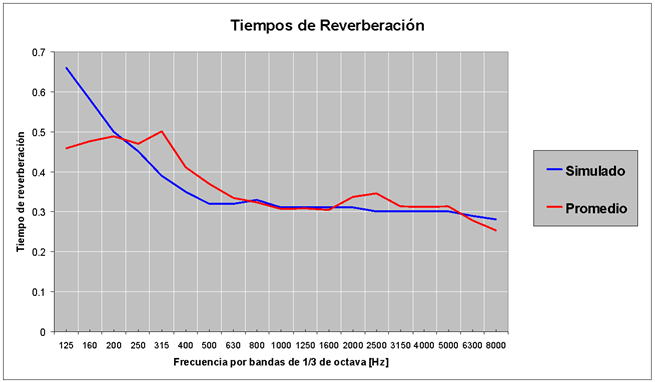
\includegraphics[scale=0.9]{Figuras/Tiempo de Reverberacion.png}
        \caption{Comparación de los tiempos de reverberación entre el promedio espacial y la simulación del Hall 4.}
        \label{fig:Tiempo de reverberacion}
    \end{figure}

    \begin{figure}[h]
        \centering
        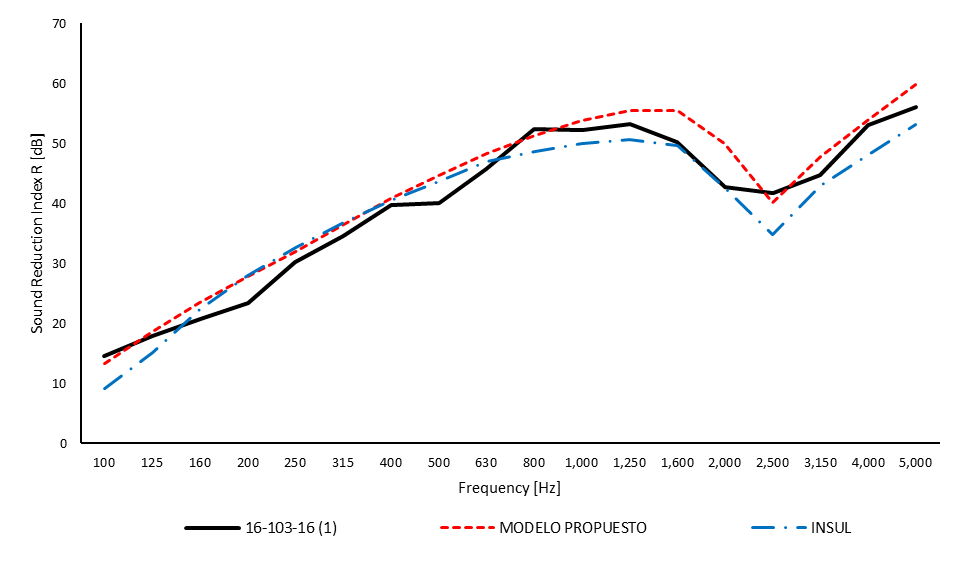
\includegraphics[scale=0.9]{Figuras/Comparacion reduccion sonora R.png}
        \caption{Comparativa de los índices de reducción sonora R entre la medición de laboratorio, la predicción del modelo propuesto y el programa INSUL para el caso 1.}
        \label{fig:Comparativa R}
    \end{figure}


\begin{table}
\centering
\begin{tblr}{
  cells = {c},
  hline{1-2,7} = {-}{},
}
\textbf{Material}  & \textbf{Espesor \\\ [mm]} & {\textbf{Densidad}\\\textbf{$[Kg/m^3]$}} & {\textbf{Young}\\\textbf{[GPa]}} & \textbf{Poisson} & {\textbf{Factor de perdidas}\\\textbf{interno}} \\
hormigon  & 50,8; 101,6; 140; 160(x2);& 2100 & 30 & 0,2 & 0,03 \\
Vidrio    & 180; 200; 220; 240              & 2500 & 71 & 0,23& 0,02  \\
placa de yeso & 6,4; 9,5; 12,7; 15.9   & 768  & 2 &  0,23& 0,01  \\
laminado  &  3.2; 6.4                       & 1250 & 3 &  0,15& 0,03  \\
HDF       &  50; 70(x4); 100                &  900 &  3.5& 0,2& 0.005
                                       
\end{tblr}
\caption{Lista de materiales utilizados en la comparativa y sus características físicas.}
\label{Tab:1}
\end{table}

\subsection*{AI 5. \textit{Bibliografía}}
Las referencias a la bibliografía utilizada deberán registrarse en el texto entre corchetes con un número arábigo (Ej [5]). La numeración debe ser consecutiva. En caso de citarse más de una referencia se hará separadas por comas dentro del corchete (Ej [5, 18]) y en caso de necesitar la cita de una sucesión consecutiva de referencias se escribirán separadas por una línea (Ej [5-11]).

La numeración correspondiente a las referencias se podrá incluir al final de la tesis (como se especifica más arriba en la descripción de la Estructura) o bien al final de cada capítulo incluyendo solamente las referencias de ese capítulo. Al utilizar las referencias por capítulo pueden quedar referencias repetidas entre capítulos; en este caso cada capítulo debe ser autocontenido con respecto a las referencias.

\end{document}

